% This is a LaTeX thesis template for Monash University.
% to be used with Rmarkdown
% This template was produced by Rob Hyndman
% Version: 6 September 2016

\documentclass{monashthesis}

%%%%%%%%%%%%%%%%%%%%%%%%%%%%%%%%%%%%%%%%%%%%%%%%%%%%%%%%%%%%%%%
% Add any LaTeX packages and other preamble here if required
%%%%%%%%%%%%%%%%%%%%%%%%%%%%%%%%%%%%%%%%%%%%%%%%%%%%%%%%%%%%%%%

\author{Xiefei Li}
\title{Revisiting the Forecast Combination Puzzle: An Empirical Study}
\studentid{30204232}
\studentemail{\href{mailto:xlii0145@student.monash.edu}{\nolinkurl{xlii0145@student.monash.edu}}}
\studentdetails{Supervisor: David T. Frazier}
\supervisoremail{\href{mailto:David.frazier@monash.edu}{\nolinkurl{David.frazier@monash.edu}}}
\def\degreetitle{Bachelor of Commerce (Honours)}
% Add subject and keywords below
\hypersetup{
     %pdfsubject={The Subject},
     %pdfkeywords={Some Keywords},
     pdfauthor={Xiefei Li},
     pdftitle={Revisiting the Forecast Combination Puzzle: An Empirical Study},
     pdfproducer={Bookdown with LaTeX}
}


\bibliography{thesisrefs}

\begin{document}

\pagenumbering{roman}

\titlepage

{\setstretch{1.2}\sf\tighttoc\doublespacing}

\clearpage\pagenumbering{arabic}\setcounter{page}{1}

\hypertarget{abstract}{%
\chapter*{Abstract}\label{abstract}}
\addcontentsline{toc}{chapter}{Abstract}

The abstract should outline the main approach and findings of the thesis and must not be more than 500 words.

\newpage

\hypertarget{acknowledgements}{%
\chapter*{Acknowledgements}\label{acknowledgements}}
\addcontentsline{toc}{chapter}{Acknowledgements}

I would like to thank my pet goldfish for \dots

\hypertarget{introduction}{%
\chapter{Introduction}\label{introduction}}

\hypertarget{research-objective}{%
\section{Research Objective}\label{research-objective}}

This thesis aims to investigate the determinants behind, and evidence for the forecast combination puzzle in various domains, and to empirically examine a general solution to the forecast combination puzzle. The combination puzzle refers to the well-known empirical finding that an equally weighted combination of forecasts generally outperforms more sophisticated combination schemes. This phenomenon is often found in the point forecast combinations but it is also the case in the density forecast combinations. Besides working with stationary time series, this research also explores how density forecast combinations perform with nonstationary time series. The empirical studies undertaken so far have focused more on pure time series settings, while there is little literature on the presence of the combination puzzle in the cross-sectional setting. The performance of density forecast combinations will be assessed via the log score function. As an additional contribution, we will assess the veracity, and applicability, of a recently proposed solution to the forecast combination puzzle suggested in \textcite{ZMFP22} and \textcite{FZMP23}.

\hypertarget{literature-review-and-motivation}{%
\section{Literature Review and Motivation}\label{literature-review-and-motivation}}

The forecast accuracy is of critical concern for forecasters and decision makers. With the evidence of dramatic improvements in the forecast accuracy, forecast combinations have attracted wide attention and contributions in the literature, both theoretical and applied \autocite{C89,T06}. More importantly, this promising approach often has a robust performance for various types of series, which is borne out by numerous empirical results \autocite{A11}. For example, \textcite{MACF82} and \textcite{SW98} demonstrated that forecast combinations perform better than individual models. MORE!!!!

Forecast combinations refer to the idea of combining multiple forecasts generated from possible models, which was originally proposed in the seminal work of \textcite{BG69}. The forecast combination methods, in general, involve producing forecasts from constituent models, and then combining them based on a rule or weighting scheme. Each scheme has different selection criteria for the ``best'' forecast combination and the corresponding weight value assigned to each model. This process can sometimes capture more meaningful characteristics of the true data generating process than using a single model, and allow us to combine the best features of different models within a single framework. Researchers have examined a variety of combination methods for both point and density forecasts over the past 50 years, see \textcite{WHLK22} for a modern literature review.

In most time series setting under which forecast combinations are employed, a striking empirical phenomenon is often observed, coined by \textcite{SW04}, as the ``forecast combination puzzle''. The puzzle is encapsulated by the fact that ``theoretically sophisticated weighting schemes should provide more benefits than the simple average from forecast combination, while empirically the simple average has been continuously found to dominate more complicated approaches to combining forecasts'' \autocite{WHLK22}. In simple words, forecast combinations obtained through weighting schemes should perform better in theory. However, the averaged forecasts are often preferred in empirical studies.

\textcite{MACF82} and \textcite{SW98} found that a simple average of the forecasts is typically more preferred with empirical evidence in the early forecast comparison studies. More recently, \textcite{SW04}, \textcite{MSA18} and \textcite{MSA20} delved more into forecast combinations, and also claimed that equally-weighted strategies are highly competitive compared with complicated weighting schemes.

In the literature, there are two possible explanations for the puzzle. One concentrates on the estimation uncertainty in combination weight (\textcite{SW98}, \textcite{SW04} and \textcite{SW09}). Complicated weighting schemes introduce variability when estimating parameters whereas the simple averaging does not require any estimation. On the other hand, \textcite{E11} and \textcite{CMVW16} explore the trade-off between bias and variance in the Mean Squared Forecast Error (MSFE). They proved that equally weighted combination is unbiased and its variance has only one component, resulting in a smaller mean squared error than a biased combination. However, this is mainly applicable to the MSFE scheme. Recently, \textcite{ZMFP22} and \textcite{FZMP23} proposed a new explanation for the puzzle in a general way by investigating the sampling variability of the forecasts induced via estimation of the constituent model forecasts (i.e., the models used to produce the forecasts). They illustrated that, asymptotically, the bias and variability mainly come from the estimation of the models used to produce the constituent model forecasts.

Most explanations for the puzzle concentrate on the error of combination weight estimation. For example, \textcite{SW04} showed that the higher average loss and instability make sophisticated weighting schemes to have inferior performance. \textcite{T06} pointed out that the success of averaging is the efficiency gains under certain assumptions whereas recursive estimation of parameters in the optimally-weighted combinations could potentially lead to biased estimators of the combination weights. On the other hand, \textcite{E11} explored the sizes of theoretical gains from optimal weights and established that the estimation error would outweigh gains if the number of forecasts is small. Later, \textcite{CMVW16} demonstrated the presence of bias and inefficiency when weights estimation is required, in comparison with the fixed-weights such as the equal weights. While various explanations for the forecast combination puzzle have been suggested over the years (see the above references), a general solution to the puzzle has so far proved elusive.

Instead of exploring the estimation error in determining optimal weights, \textcite{ZMFP22} investigated the sampling variability in estimating constituent models and the main determinant of forecast combination performance. They illustrated that, asymptotically, the bias and variability mainly come from the estimation of parameters in the constituent models, rather than the weight estimation. This new insight motivates \textcite{FZMP23} to propose a most general solution to the puzzle. They demonstrated that, in theory, the puzzle is evident due to the way of producing forecast combinations. Furthermore, a process of eliminating the puzzle is also suggested, which is to produce forecasts by estimating parameters and weights simultaneously, if feasible. Under this approach, the sophisticated weighting schemes should (asymptotically) be superior.

\begin{table}[ht]
\centering
\begin{tabular}{lcccccccc}
\toprule
&
\multicolumn{2}{c}{Both Correct} &
\multicolumn{2}{c}{Marginal Miss. } &
\multicolumn{2}{c}{Copula Miss. } &
\multicolumn{2}{c}{Both Miss. }
\\

& {bt} & {bp} & {bt} & {bp} & {bt} & {bp} & {bt} & {bp} \\
\midrule
Cut1 & $\surd$ & $\surd$ & $\times$ & $\times$ & $\surd$ & $\times$ & $\times$ & $\times$ \\
Cut2 & $\surd$ & $\surd$ & $\times$ & $\surd$ & $\times$ & $\times$ & $\times$ & $\times$ \\

\bottomrule
\end{tabular}
\caption{The column headings refer to the four different classes of DGPs analyzed in our study. Both Correct implies that both parameteric models are correct; Marginal Miss. implies that the marginal models are misspecified, but the copula model is correct; Copula Miss. is the case where the copula model is misspecified but the marginal models are correctly specified, and Both Miss. refers to the case where both models are misspecified. Cut$_1$ refers to the cut posterior where we cut away the marginal parameters vt, while Cut$_2$ refers to the cut posterior where we cut away the copula parameters bp using the rank likelihood approach. The parameters vt and bp refer to calibration of that specific parameter  under the different combinations of cut posterior, and DGP. The ``$\surd$`` indicates (asymptotically) correct calibration, while ``$\times$`` denotes (possibly) inaccurate calibration.}
\label{tab:1}
\end{table}

There are 3 sets of two-model combination and the log predictive score of each combination is generated according to \ref{eqn:LS} with the value of weight changing by 0.01 every time. Table \ref{tab:2} shows the estimated weights and combination log scores.

The goal of this thesis is two-fold: first, to search for empirical evidence of the combination puzzle in settings outside of the usual time series in which it has been found; second, to test the empirical veracity of the theoretical solution to the puzzle found in \textcite{FZMP23}, both within, and outside of, the standard time series setting where the puzzle is often observed.

we may be able to answer the question: why does the simple average work so well - good in different ways for nonstationary time series

Under what conditions, the puzzle will exist

We start with modelling nonstationary time series with high volatility without removing the unit root. The forecast combinations between the in-sample period and the out-of-sample period are not similar.

Even though there is a widespread literature among different pure time series settings, not much attention has been put on the cross-sectional datasets. We investigate the forecasting performance of simulated cross-sectional data

We illustrate that the presence of the forecast combination puzzle is determined by at least 4 elements in the two-model pool case with simulated cross-sectional data and mis-specified models. In this special case, the puzzle can be avoided with

The puzzle is sensible with the sample size, the true value of parameters, the correlation between regressors, the difference variance of each regres

variance difference

sample size
slit proportion
true value of

The first goal of this paper is to construct linear density forecast combinations with parametric models. The results are anticipated to reveal that forecast combinations can deliver improved accuracy over single models, but are not necessarily superior to forecasts obtained from the equally weighted combination.

The next goal is to estimate the unknown parameters of the constituent models and the weight in a single step, and to compare the accuracy of forecasts based on these combinations against the usual combinations process, as well as the equally weighted combination. To measure differences between these forecasts, we will eventually employ forecast accuracy tests, of the type derived in \textcite{W96}, which measure out-of-sample differences between forecasts.

The first goal of this paper is to construct linear density forecast combinations with parametric models. In addition to point forecasts, the use of density forecasts can offer forecasters or decision markers a broader and more comprehensive view of the target variable (see section 2.6.1. of \textcite{FTP22} for related contributions). The results are anticipated to reveal that forecast combinations can deliver improved accuracy over single models, but are not necessarily superior to forecasts obtained from the equally weighted combination.

\hypertarget{method}{%
\chapter{Methodology}\label{method}}

In the literature, there are several definitions of combinations. We focus on the combination of multiple forecasts from independent models for a given dataset, which is often performed in two stages:

\begin{enumerate}
\def\labelenumi{\arabic{enumi}.}
\item
  producing separate point or probabilistic forecasts for the next time point using observed data and constituent models, and
\item
  combining forecasts based on one of the accuracy criteria.
\end{enumerate}

Before explaining further details, the following notation will be used throughout the paper. A vector time series \(\textbf{y}_t\) with a total of \(T\) observations will be divided proportionally into two parts, an in-sample period \(R\) and an out-of-sample period \(P\). The realization of a target variable \(y\) at time \(t\) is denoted as \(y_{t}\). Its future values after the in-sample period is denoted as \(y_{\small{R+h}}\), where \(h\) is the forecast horizon and \(h>0\). The information set at time t, \(\mathcal{F}_t\), is comprised of all observed (and known) realizations of \(y\) up to time t, i.e., \(\mathcal{F}_t = \{y_1, y_2, .., y_t\}\).

The choice and specification of constituent models are determined by the features of the in-sample data. For each model, the error term is assumed to be independent and normally distributed so that the Maximum Likelihood Estimation (MLE) method can be applied to generate the estimators of unknown parameters. Given the log likelihood function of in-sample period for each model, the corresponding estimates are obtained when they maximize that function and then held fixed for the following procedures. The optimal combination is then constructed with the estimated weight of each model that delivers the best accuracy.

A parametric model \(M\) determines the conditional probability density for \(\textbf{y}_t\), denoted by \(f(y_t|\mathcal{F}_{t-1}, \theta_M, M)\), given unknown parameters \(\theta_M\) and all the past information \(\mathcal{F}_{t-1}\). The choice and specification of constituent models vary by the features of the in-sample data. For each model, the error term is assumed to be independent and normally distributed so that the Maximum Likelihood Estimation (MLE) method can be applied to generate the estimators of unknown parameters, i.e., \(\hat\theta_M = \underset{\theta_M}{\arg\max} \sum^R_{t=1} log f(y_t|\mathcal{F}_{t-1}, M)\). Given the log likelihood function of in-sample period for each model, the corresponding estimates are obtained when they maximize that function and then held fixed for the following procedures.

One thing to clarify is that we do not consider the properties of estimators, so model misspecification will not ruin the results.

\hypertarget{density-combinations}{%
\section{Density combinations}\label{density-combinations}}

\hypertarget{linear-pooling}{%
\subsection{Linear pooling}\label{linear-pooling}}

Consider the case of only two competing probability densities, undoubtedly, densities can be combined in many ways; see Section 3 of \textcite{WHLK22} for many popular means of probabilistic combination. One of the commonly used approaches is the ``linear opinion pool'': aggregate constituent weighted densities in a linear form \autocite{BG69,HM07,GA11}. For the \texttt{two-model} pools, constituent densities \(f_1(y_t)\) and \(f_2(y_t)\) are combined as follows:

\begin{equation}
\label{eqn:LC1}
f(y_t) = w \ f_1(y_t | \mathcal{F}_{t-1}, \hat\theta_{M1}, M_1) + (1-w) f_2(y_t | \mathcal{F}_{t-1}, \hat\theta_{M2}, M_2)
\end{equation}

where \(w\) is the non-negative weight allocated to the probability density derived from the first model. Through this construction, the sum of two weights is implied to be 1, which is a necessary and sufficient condition for \(f(y_t)\) to be a proper density function \autocite{GA11}.

\hypertarget{log-socring-rules}{%
\subsection{Log socring rules}\label{log-socring-rules}}

Following the literature on density evaluation, our initial analysis will focus on using the log score function to measure the accuracy of our density forecasts; see, e.g., \textcite{GA11} for a discussion on log score and its use in density forecasting. For each individual model \(M\), the log score over the sample \(t = 1, \dots, T\) is:

\begin{equation}
\label{eqn:LS1}
LS = \sum^T_{t=1} log \ f(y_t| \mathcal{F}_{t-1}, \hat\theta_M, M).
\end{equation}

The ``optimal'' linear combination is identified to produce the most accurate forecasts when the set of weights maximizes the log score function of two densities over the in-sample \(t = 1, 2, \dots, R\).

\begin{equation}
\label{eqn:LS2}
\hat{w}_{\text{opt}} = \underset{w}{\arg\max} \sum^R_{t=1} log \Big[ w \ f_1(y_t| \mathcal{F}_{t-1}, \hat\theta_{M1}, M_1) + (1-w) \ f_2(y_t| \mathcal{F}_{t-1}, \hat\theta_{M2}, M_2)\Big]
\end{equation}

Thus, the log predictive score over the forecast horizon \(h = 1, 2, \dots, P\) (i.e., the out-of-sample period) is:

\begin{equation}
\label{eqn:LS3}
LPS = \sum^T_{t = R+1} log \Big[ \hat{w}_{\text{opt}} \ f_1(y_t| \mathcal{F}_{t-1}, \hat\theta_{M1}, M_1) + (1- \hat{w}_{\text{opt}}) \ f_2(y_t| \mathcal{F}_{t-1}, \hat\theta_{M2}, M_2)\Big].
\end{equation}

\hypertarget{point-combinations}{%
\section{Point combinations}\label{point-combinations}}

For time series with seasonal patterns, we follow \textcite{BG69} and \textcite{SW09}, and consider the combination of pairs of point forecasts for the ease of calculation. Same as \textcite{SW09}, the mean squared forecast error (MSFE) is adopted to measure the point forecast accuracy.

\hypertarget{linear-combination}{%
\subsection{Linear combination}\label{linear-combination}}

Similar to the density case, point predictions from two models, \(\hat y_{1t}\) and \(\hat y_{2t}\), are aggregated linearly:

\begin{equation}
\label{eqn:PC1}
\hat y_t = w \ \hat y_{1t} + (1-w) \ \hat y_{2t}
\end{equation}

where \(w\) is the non-negative weight allocated to the point prediction generated from the first model.

\hypertarget{mean-squared-forecast-error-msfe}{%
\subsection{Mean squared forecast error (MSFE)}\label{mean-squared-forecast-error-msfe}}

The MSFE is defined as

\begin{equation}
\label{eqn:MSFE1}
\frac{1}{P} \sum^T_{t=R+1} (y_t - \hat y_t)^2.
\end{equation}

The ``optimal'' set of weights satisfies that it minimizes the MSFE among all other possible sets.

\hypertarget{empirical-results}{%
\chapter{Empirical Results}\label{empirical-results}}

\hypertarget{pure-time-series-setting-sp-500}{%
\section{Pure time series setting (S\&P 500)}\label{pure-time-series-setting-sp-500}}

Reconsidering the example in Section 3 of \textcite{GA11}, the data we use is the daily Standard and Poor's (S\&P) 500 index from February 11, 2013 to February 10, 2023 (10 years in total), retrieved from the \textcite{SP500}. The S\&P500 index dataset has a total of 2519 (\(T\)) observations and is partitioned into two periods with a rough proportion. The in-sample period contains the first 60\% of the data (\(R = 1511\)), which is used to estimate all unknown parameters, including the optimal weight. The remaining 40\% (\(P = 1008\)) becomes the out-of-sample period to evaluate the forecast performance.

We will investigate the presence of the forecast combination puzzle when fitting the nonstationary data and the stationary data. Constituent models come from commonly used model types, which are autoregressive integrated moving average (ARIMA), exponential smoothing (ETS), and linear regression model with ARIMA errors. Detailed model specifications for each case will be clarified in the corresponding section.

To start with,

We choose \(j=1,\cdots,M\), with \(M=3\) prediction models to study the performance of density predictions across sets of \texttt{two-model} pools. Each of the \(j\) predictive model has a conditional Gaussian density, which takes the form \(f^{(j)}(y)=f_j(y_t|\mathcal{F}_{t-1})=N\{y_t; \mu_j, \sigma^2_j\}\), where \(N\{x; \mu, \sigma^2\}\) denotes the normal probability density function evaluated at value \(x\) with mean \(\mu\) and variance \(\sigma^2\). The notation \(\mathcal{F}_{t-1}\) denotes all information available at time \(t-1\), and we assume that the conditional mean and variance of the models are, up to unknown parameters, known at time \(t-1\).

\hypertarget{fitting-the-nonstationary-time-series}{%
\subsection{Fitting the nonstationary time series}\label{fitting-the-nonstationary-time-series}}

To reduce the level of variability, we take a natural logarithm of the S\&P 500 index and fit three candidate models directly without removing its stochastic trend.

\begin{enumerate}
\def\labelenumi{\arabic{enumi}.}
\item
  Model 1: ARIMA(1,1,1) model with an intercept of the natural logarithm of S\&P 500 index.
  \begin{equation*}
  log(y_t) = c + log(y_{t-1}) + \phi_1\big[log(y_{t-1})-log(y_{t-2})\big] + \epsilon_t + \theta_1\epsilon_{t-1}
  \end{equation*}
\item
  Model 2: ETS(M,N,N) model of the natural logarithm of S\&P 500 index.
  \begin{align*}
  log(y_t) &= \ell_{t-1} (1+\epsilon_t) \\
  \ell_t &= \ell_{t-1} (1+\alpha \epsilon_t) \\
  \end{align*}
\item
  Model 3: A linear regression model of the natural logarithm of the S\&P 500 index and ARIMA(1,0,0) errors.
  \begin{align*}
  log(y_t) &= \beta_0 + \beta_1 t + u_t \\
  u_t &= \phi_1 u_{t-1} + \epsilon_t
  \end{align*}
\end{enumerate}

The error term, \(\epsilon_t\), in each model is assumed to be independent and normally distributed with a zero mean and a constant variance.

\begin{table}[ht]
  \centering
  \caption{Log predictive score of density forecasts combination under two-model pools}
    \begin{tabular}{llllll}
    \toprule
          & ARIMA(1,1,1) & ETS(M,N,N) & LR \\
    \midrule
    ARIMA(1,1,1) & \textit{-5911.1974} & -5839.3045 & -5842.7634 \\
    ETS(M,N,N) & 0.45  & \textit{-5883.9697} & -5881.7790 \\
    LR & 0.43  & 0.08  & \textit{-5881.7970} \\
    \bottomrule
    \multicolumn{4}{l}{\footnotesize The diagonal entries contains individual log score.}\\
    \multicolumn{4}{l}{\footnotesize The log scores for combination pools are located above the diagonal.}\\
    \multicolumn{4}{l}{\footnotesize Entries below diagonal show the estimated weight of the model in that column in the two-model pool.}\\
    \end{tabular}
  \label{tab:2}
\end{table}

There are 3 sets of two-model combination and the log predictive score of each combination is generated according to \ref{eqn:LS} with the value of weight changing by 0.01 every time. Table \ref{tab:2} shows the estimated weights and combination log scores.

We focused on the combination of two individual forecasts for two reasons, which in most cases apply for the prediction of business figures in enterprises. Typically, a judgmental forecast and one that is derived using purely statistical means are available and corporate planning can be based on one of the forecast or a combination of both forecasts, where additional forecasts cannot be expected to introduce as much additional information. Furthermore, focusing on the two-forecast case allowed us to provide a variety of in-depth analyses. The challenge of extending the model and the decision boundaries to a larger, arbitrary number of forecasts is subject to future research.

All unknown parameters are estimated by maximizing the likelihood function using the in-sample period data. Once the estimated are obtained, they are held fixed for the density evaluations. For each model, I generate the predictive densities at every future time point of S\&P 500 returns (\(h=1,2,...,P\)) given that all past information is known. In order to make a comparison between each pair of these models, the log of S\&P 500 returns will be ``back-transformed'' by evaluating with the log normal density function.

\hypertarget{fitting-the-stationary-time-series}{%
\subsection{Fitting the stationary time series}\label{fitting-the-stationary-time-series}}

\hypertarget{simulation-results}{%
\chapter{Simulation Results}\label{simulation-results}}

\hypertarget{pure-cross-sectional-setting}{%
\section{Pure cross-sectional setting}\label{pure-cross-sectional-setting}}

Given that the forecast combination can greatly improve the forecast accuracy, this idea of model combination can also be applied to the cross-sectional setting. Rather than forecasting future value, cross-sectional data often helps to better understand the individual behavior and decision-making with changing attributes.

A simulated cross-sectional dataset is designed to study how related elements in the linear regression model affect the presence of the puzzle, as well as the performance of density combinations. In line with previous notations but under the cross-sectional setting, the subscript \texttt{t} will change to \texttt{i} to represent each individual observation.

CHECK MOTIVATION!!!!

\hypertarget{experimental-design}{%
\subsection{Experimental design}\label{experimental-design}}

The true data-generating process (DGP) is assumed to be a classic linear regression model with only two exogenous and correlated regressors, which satisfies all classical assumptions:

\begin{equation}
\label{eqn:DGP}
y_i = \beta_0 + \beta_1 x_{1i} + \beta_2 x_{2i} + e_i, \ \ e_i \stackrel{i.i.d}{\sim} N(\mu_e,\sigma^2_e) \\
\end{equation}

where \(i\) represents each observation.

The initial set-up has 15000 (N) artificial cross-sectional observations generated from \ref{eqn:DGP} with \(E[x_{1i}] = E[x_{2i}] = 0\), \(Var(x_{1i}) = Var(x_{2i}) = 1\), \(Cov(x_{1i}, x_{2i}) = 0.7\), \(\pmb{\beta} = (\beta_0, \beta_1, \beta_2)' = (1,2,2)'\), \(\mu_e = 5\) and \(\sigma^2_e=10\).

Following the methodology in Section \ref{method}, the data will be divided into an in-sample period (roughly 60\%) for estimation and an out-of-sample period for accuracy evaluation. We propose two mis-specified models to generate density forecasts with each only contains one of the regressors. Assume Model 1 includes only \(x_{1i}\) as the regressor and the other model, Model 2, includes only \(x_{2i}\) as the regressor. The density forecast combinations will follow the construction of \texttt{two-model} pools and be evaluated by the log score functions.

\begin{itemize}
\item
  Sample size is \(N=15000\)
\item
  \(E[x_{1i}] = E[x_{2i}] = 0\)
\item
  \(Var(x_{1i}) = Var(x_{2i}) = 1\)
\item
  \(Cov(x_{1i}, x_{2i}) = 0.7\)
\item
  The true value of \(\pmb{\beta} = (\beta_0, \beta_1, \beta_2)' = (1,2,2)'\)
\item
  \(\mu_e = 5\) and \(\sigma^2_e=10\)
\end{itemize}

\begin{figure}[ht]
\centering
\includegraphics[scale=0.6]{figures/Sample_Size_15000.pdf}
\caption{Two curves refer to the in-sample (left) and out-of-sample (right) performance of density combinations with artificial cross-sectional data under the initial set-up. The x-axis represents the weight assignment on the Model 1 and the y-axis indicates the log score for each density combination. The orange dot represents the optimal set of weights and the corresponding log predictive score in each case, while the blue dot indicates the forecast performance of the simple averaging method. The green dot, as a reference, refers to the maximum point of the out-of-sample curve.}
\label{fig:ss15000}
\end{figure}

Figure \ref{fig:ss15000} clearly reflects that when the sample size is large enough, the simple average of predicted densities, indicated by the blue dot, can retain the forecast accuracy with a small difference in the log predictive score, compared with the optimal combination indicated by the orange dot. This is an evidence of facing forecast combination puzzle. Given the puzzle, we can change the true value of relevant elements one at a time while holding all others constant, and then summarize the conditions under which the puzzle is likely to be evident.

\begin{itemize}
\tightlist
\item
  \bf{Sample Size}
\end{itemize}

\begin{figure}[ht]
\centering
\includegraphics[scale=0.35]{figures/Sample_Size_100-10000.png}
\caption{Three columns refer to the cases when $N=100$, $N=1000$, and $N=10000$ respectively while keeping all others constant as the initial set-up. The upper graphs represent the in-sample combination performance and the bottom graphs represent the out-of-sample combination accuracy. The meanings of colored dots are the same as those in Figure \ref{fig:ss15000}.}
\label{fig:ss}
\end{figure}

First, it is noticeable that the performances of in-sample and out-of-sample combinations have completely different shapes or features when \(N=100\) but are gradually similar when \(N=1000\) and \(N=10000\). In the \(N=100\) case, we completely prefer Model 1 to fit the training set, however, the Model 1 becomes the worse choice for the test set. Although the averaged density forecast performs much better than the combination recommended by the optimal weight, the accuracy could still be of concern. Second, the orange dot is approaching to the green dot when the sample size increases. This implies that the model combination which fits the in-sample well does not necessarily generate better forecasts when the sample size is small. In this case, it is conservative to use averaged forecasts.

To be more rigorous, the puzzle becomes notable when the sample size is larger than 9000.

When we have a small dataset, it is not representative of the whole population, so the model estimation involves more randomness and is highly influenced by potential outliers. There is also a possibility of overfitting when the training and test sets have distinct patterns.

Given a large enough dataset and two equally good models

\begin{itemize}
\tightlist
\item
  \bf{Sign and Magnitude of $\pmb{\beta}$}
\end{itemize}

Next, the sample size is set to be 10000 so that it is large enough to reveal the puzzle. Consider the change in sign and magnitude of \(\beta_1\) and \(\beta_2\).

\begin{figure}[ht]
\centering
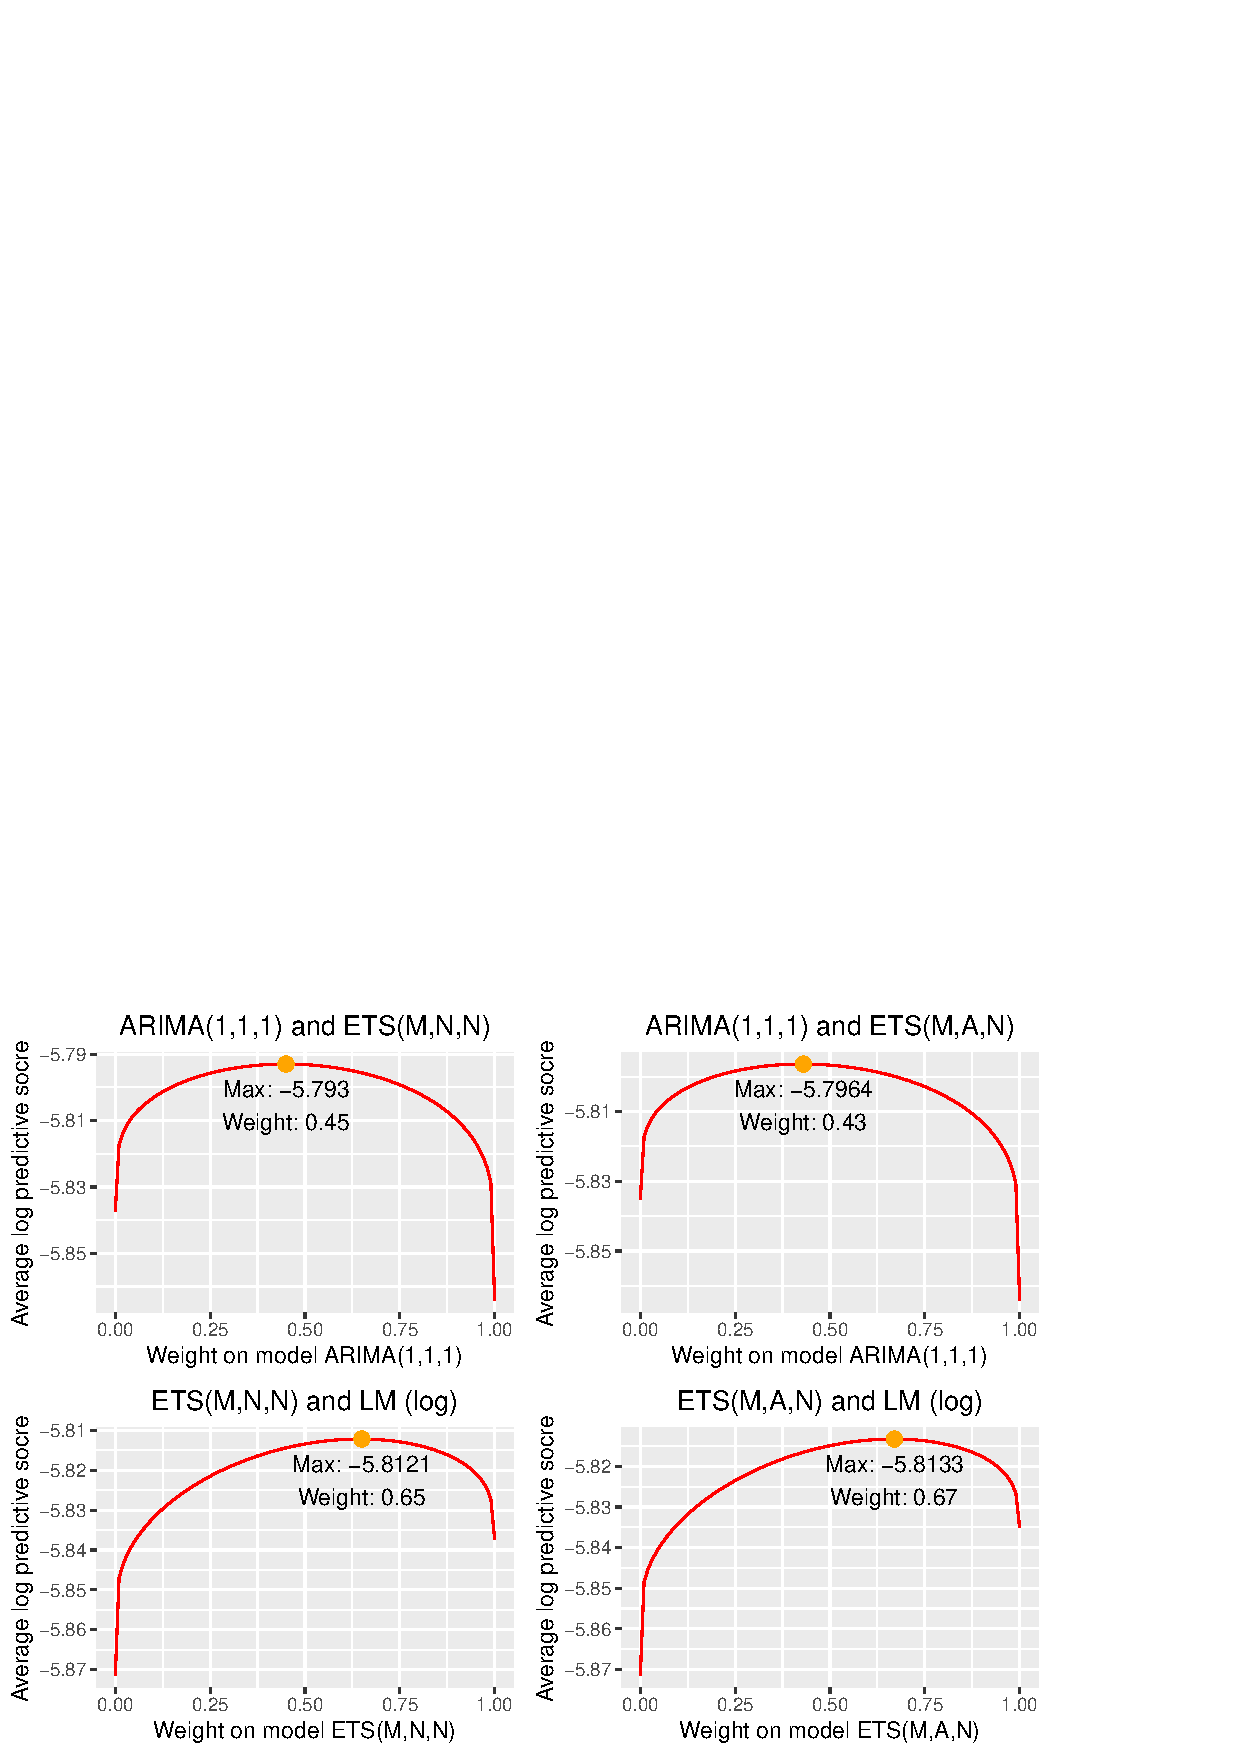
\includegraphics[scale=0.35]{figures/best4.pdf}
\caption{Three columns refer to the cases when }
\label{fig:sign}
\end{figure}

\begin{figure}[ht]
\centering
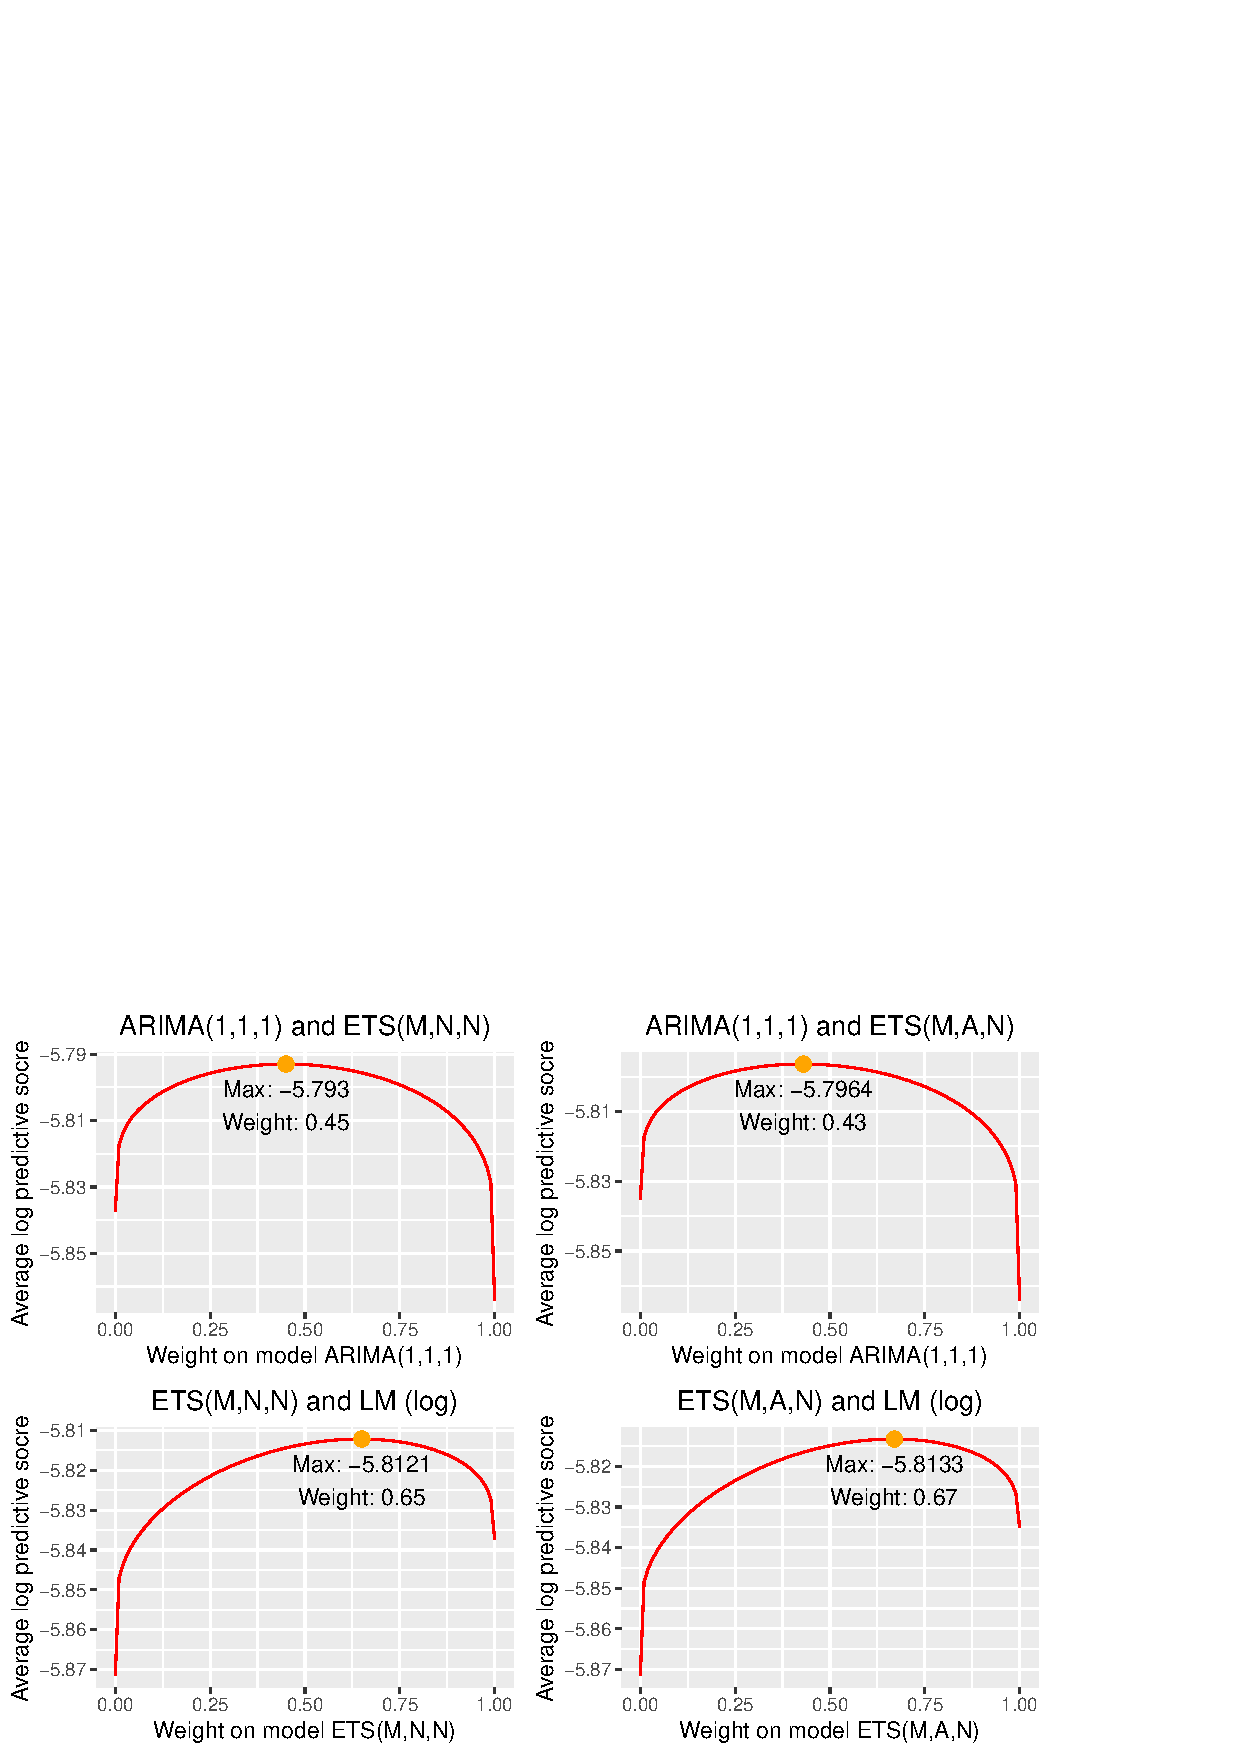
\includegraphics[scale=0.35]{figures/best4.pdf}
\caption{Three columns refer to the cases when }
\label{fig:magnitude}
\end{figure}

The puzzle is highly sensitive to the absolute difference between two parameters but insensitive to the sign. If the absolute difference is large enough, generally more than half of the smaller coefficient, it is hard to observe the puzzle and the optimal combination always wins.

The magnitude of each coefficient acts like the weight of each regressor on the dependent variable.
The one which includes the more important regressor will be more favoured with a higher weight in the forecast combination

\begin{itemize}
\tightlist
\item
  \bf{Variance of regressors}
\end{itemize}

larger variance, more variation to explain y, more favored

Variance of the error term will influence the log score value
Pattern is hard to determine

Estimates based on equation (2) need not satisfy, as noted in section 2.1, especially if the correlation between the competing forecast errors is large and positive, and we consider two possibilities. One is to use the observed point estimate; the second, following widespread practice, is to replace an estimate out- side this range by the nearest boundary value, 0 or 1 as appropriate. There are then four combined forecasts whose MSFEs are calculated over the last P observations: three weighted averages, in turn using and the observed and truncated, and the simple average using k=0.5. The estimation cost of each weighted average is expressed as the percentage increase in MSFE above that of the simple average,

\vspace{0.3cm}

\begin{figure}[ht]
\centering
\caption{The highest four log predictive scores of weighted two-model combinations for S\&P 500 index predictive densities.}
\includegraphics{figures/Sample_Size_100.pdf}
\begin{flushleft}
{\footnotesize The weights on the first model is in the x-axis and the corresponding log predictive scores are on the y-axis. Constituent models are stated in the title. The orange point represent the highest log score of a specific combination. Its value and the corresponding estimated weight are noted below.}\\
\end{flushleft}
\label{fig:ss100}
\end{figure}

Figure \ref{fig:ss100} illustrates

\begin{figure}
\centering
\caption{The highest four log predictive scores of weighted two-model combinations for S\&P 500 index predictive densities.}
\includegraphics{figures/Sample_Size_1000.pdf}
\label{fig:ss1000}
\end{figure}

\hypertarget{discussion}{%
\chapter{Discussion}\label{discussion}}

\hypertarget{research-objective-1}{%
\section{Research Objective}\label{research-objective-1}}

\appendix

\hypertarget{appendix}{%
\chapter{Appendix}\label{appendix}}

All analyses were performed using R Statistical Software (R version 4.2.1 (2022-06-23))

Packages used are \texttt{tidyverse} \autocite{tidy19}, \texttt{dplyr} \autocite{dplyr23}, and \texttt{fpp3} \autocite{fpp23}.

\[\begin{aligned}
M_1: log(y_t) &= \phi_{0,1} + log(y_{t-1}) + \phi_{1,1}log(y)_{t-1} + \theta_{1,1}\epsilon_{t-1} + \epsilon_{t,1} \ \ \ \ \epsilon_t \stackrel{i.i.d.}{\sim} N(0,\sigma_1^2) \\
M_2: y_t &= \ell_{t-1,2}(1+\epsilon_{t,2}) \\
  \ell_{t,2} &= \ell_{t-1,2}(1+\alpha_2\epsilon_{t,2}) \\
M_3: y_t &= (\ell_{t-1}+b_{t-1}) (1+\epsilon_{t,3}) \\
  \ell_t &= \ell_{t-1}(1+\alpha\epsilon_{t,2}) \\
M_4&: y_t = \\
M_5&: y_t = 
\end{aligned}\]

\begin{equation}
  y_t - y_{t-4} = \beta (x_t-x_{t-4}) + \gamma (z_t-z_{t-4}) + \phi_1 (y_{t-1} - y_{t-5}) + \Theta_1 \varepsilon_{t-4} + \varepsilon_t
\end{equation}

\textcite{fpp3}

\printbibliography[title={Reference}]




\end{document}
